\documentclass[11pt,a4paper]{article}
\usepackage{graphicx}
\usepackage{wrapfig}
\usepackage{caption}
\usepackage{geometry}
\usepackage{titlesec}
\usepackage{parskip}
\usepackage{xcolor}
\usepackage{tikz}
\geometry{margin=1in}
\setlength{\parindent}{0pt}
\pagestyle{empty}
\usepackage{tcolorbox}
\usepackage{fancyhdr}
\usepackage{array}
\usepackage{amsmath,amssymb}
\usepackage{microtype}
\usepackage[utf8]{inputenc}
\usepackage{enumitem}
\geometry{top=1in, bottom=1in, left=1in, right=1in}




% Define custom colors
\definecolor{blueheader}{RGB}{0,112,192}
\definecolor{textcolor}{RGB}{0,0,0}

% Section formatting (for trigonometric ratios title)
\titleformat{\section}
  {\normalfont\large\bfseries\color{blueheader}}{\thesection}{1em}{}

\begin{document}
\begin{figure}[h!]
    \begin{minipage}{0.45\textwidth}  % Set the width of the image
        \includegraphics[width=\textwidth]{/storage/emulated/0/vinod/IMG-20250515-WA0024.png}  % Replace 'image.png' with your image file name
    \end{minipage} \hfill
    \begin{minipage}{0.45\textwidth}  % Set the width of the text block
        \textbf{Name : Kiran Kumar Reddy L} \\
    \textbf{id : cometfwc027} \\
  \textbf{Date : 15th may 2025}
    \end{minipage}
\end{figure}
\begin{center}
    \includegraphics[width=1.5cm]{img6.png} \\[1em]
    \hspace{6em}{\LARGE \textcolor{cyan}{\textbf{INTRODUCTION TO}}}\\
    \vspace{1em}
   \hspace{8em} {\LARGE \textcolor{cyan}{\textbf{TRIGONOMETRY}}}
\vspace{-2cm}
\begin{flushright}
   \begin{minipage}{0.2\textwidth}
   \hspace{4em}\framebox(50pt,50pt){\fontsize{30}{30}\selectfont\textbf{8}}
    \end{minipage}
\end{flushright}
    \noindent\textcolor{cyan}{\rule{\textwidth}{1pt}}
    \item\ \textcolor{cyan}{There is perhaps nothing which so occupies the\\
    middle position of mathematics as trigonometry.}\\
    \hspace{2cm} \textbf{-J.F. Herbert (1890)}
\end{center}

\vspace{1em}
{\large \textcolor{cyan}{\textbf{8.1 Introduction}}}

\vspace{0.5em}
You have already studied about triangles, and in particular, right triangles, in your earlier classes. Let us take some examples from our surroundings where right triangles can be imagined to be formed. For instance:

\vspace{1em}

% Example 1: Paragraph + Fig 8.1
\noindent
\begin{minipage}[t]{0.6\textwidth}
\raggedright
\vspace{-5cm}
\textbf{1.} Suppose the students of a school are visiting Qutub Minar. Now, if a student is looking at the top of the Minar, a right triangle can be imagined to be made, as shown in Fig. 8.1. Can the student find out the height of the Minar without actually measuring it?
\end{minipage}%
\hfill
\begin{minipage}[t]{0.35\textwidth}
\centering
\includegraphics[width=\linewidth]{img7.png}\\
\end{minipage}

\vspace{2em}

% Example 2: Paragraph + Fig 8.2
\noindent
\begin{minipage}[t]{0.6\textwidth}
\raggedright
\vspace{-5cm}
\textbf{2.} Suppose a girl is sitting on the balcony of her house located on the bank of a river. She is looking down at a flower pot placed on a stair of a temple situated nearly on the other bank of the river. A right triangle is imagined to be made in this situation as shown in Fig. 8.2. If you know the height at which the person is sitting, can you find the width of the river?
\end{minipage}%
\hfill
\begin{minipage}[t]{0.35\textwidth}
\centering
\includegraphics[width=\linewidth]{img8.png}\\
\end{minipage}
\vspace{2em}
\begin{center}
2019-20
\end{center}
\pagestyle{empty}
\color{textcolor}

% ---------- Header ----------
\vspace*{5em}
\begin{flushright}
    \textbf{\textsf{\textcolor{cyan}{MATHEMATICS}}}

\end{flushright}
\vspace{-0.2cm}
\noindent\textcolor{cyan}{\rule{\textwidth}{1pt}}


\vspace{1em}

% ---------- First Paragraph with Fig. 8.3 ----------
\begin{wrapfigure}{r}{0.43\textwidth}
  \centering
  \vspace{-1em}
  \includegraphics[width=0.4\textwidth]{img1.png}
  \caption*{\small Fig. 8.3}
\end{wrapfigure}

3. Suppose a hot air balloon is flying in the air.A girl happens to spot the balloon in the sky and runs to her mother to tell her about it. Her mother rushes out of the house to look at the balloon. Now when the girl had spotted the balloon initially it was at point A. When both the mother and daughter came out to see it, it had already travelled to another point B. Can you find the altitude of B from the ground?

\vspace{1em}

In all the situations given above, the distances or heights can be found by using some mathematical techniques, which come under a branch of mathematics called \textbf{‘trigonometry’}. The word ‘trigonometry’ is derived from the Greek words \textit{‘tri’} (meaning three), \textit{‘gon’} (meaning sides), and \textit{‘metron’} (meaning measure). In fact, trigonometry is the study of relationships between the sides and angles of a triangle.

The earliest known work on trigonometry was recorded in Egypt and Babylon. Early astronomers used it to find out the distances of the stars and planets from the Earth. Even today, most of the technologically advanced methods used in Engineering and Physical Sciences are based on trigonometrical concepts.

\vspace{0.5em}
In this chapter, we will study some ratios of the sides of a right triangle with respect to its acute angles, called \textbf{trigonometric ratios of the angle}. We will restrict our discussion to acute angles only. However, these ratios can be extended to other angles also. We will also define the trigonometric ratios for angles of measure $0^\circ$ and $90^\circ$. We will calculate trigonometric ratios for some specific angles and establish some identities involving these ratios, called \textbf{trigonometric identities}.
\vspace{-0.5em}
\section*{8.2 Trigonometric Ratios}


% ---------- Fig. 8.4 with Paragraph ----------
\begin{wrapfigure}{r}{0.4\textwidth}
  \centering
  \vspace{-1.5em}
  \includegraphics[width=0.3\textwidth]{img2.png}
  \caption*{\small Fig. 8.4}
\end{wrapfigure}

In Section 8.1, you have seen some right triangles imagined to be formed in different situations.

Let us take a right triangle ABC as shown in Fig. 8.4.

Here, $\angle CAB$ (or, in brief, angle A) is an acute angle. Note the position of the side $BC$ with respect to angle A. It faces $\angle A$. We call it the \textit{side opposite to angle A}. $AC$ is the \textit{hypotenuse} of the right triangle and the side $AB$ is a part of $\angle A$. So, we call it the \textit{side adjacent to angle A}.



% Section title
\vspace{10em}
\section*{Introduction to Trigonometry}
% Blue Horizontal Line
\vspace{-0.2cm}
\noindent\textcolor{cyan}{\rule{\textwidth}{1pt}}

% Quote section
\vspace{0.3cm}

% Wrap figure aligned to the right

  

\noindent
Note that the position of sides change when you consider angle C in place of A (see Fig. 8.5).
\begin{wrapfigure}
{r}{0.4\textwidth}
\includegraphics[width=1.3\linewidth]{img3.png} 
\label{fig:wrapfig}
\end{wrapfigure}


You have studied the concept of ‘ratio’ in your earlier classes. We now define certain ratios involving the sides of a right triangle, and call them trigonometric ratios.

\textbf{The trigonometric ratios} of the angle A in right triangle ABC (see Fig. 8.4) are defined as follows:

\[
\sin \angle A = \frac{\text{side opposite to angle A}}{\text{hypotenuse}} = \frac{BC}{AC}
\]

\[
\cos \angle A = \frac{\text{side adjacent to angle A}}{\text{hypotenuse}} = \frac{AB}{AC}
\]

\[
\tan \angle A = \frac{\text{side opposite to angle A}}{\text{side adjacent to angle A}} = \frac{BC}{AB}
\]

\[
\csc \angle A = \frac{1}{\sin \angle A} = \frac{\text{hypotenuse}}{\text{side opposite to angle A}} = \frac{AC}{BC}
\]

\[
\sec \angle A = \frac{1}{\cos \angle A} = \frac{\text{hypotenuse}}{\text{side adjacent to angle A}} = \frac{AC}{AB}
\]

\[
\cot \angle A = \frac{1}{\tan \angle A} = \frac{\text{side adjacent to angle A}}{\text{side opposite to angle A}} = \frac{AB}{BC}
\]
The ratios defined above are abbreviated as sin A, cos A, tan A, cosec A, sec A and cot A respectively. Note that the ratios \textbf{cosec A, sec A and cot A} are respectively, the reciprocals of the ratios sin A, cos A and tan A.

\[
\tan A = \frac{BC}{AB} = \frac{BC}{AC} \cdot \frac{AC}{AB} = \frac{\sin A}{\cos A}, \quad \cot A = \frac{\cos A}{\sin A}
\]

So, the \textbf{trigonometric ratios} of an acute angle in a right triangle express the relationship between the angle and the length of its sides.

Why don’t you try to define the trigonometric ratios for angle C in the right triangle? (See Fig. 8.5)

\vfill
\begin{center}
2019-20
\end{center}



% Page number and Mathematics title
\noindent \color{cyan} 176 \hfill \textsc{Mathematics}

% Blue line below Mathematics
\noindent \color{cyan} \rule{\linewidth}{0.5pt}

\vspace{0.5cm}

% First paragraph inside blue box with Aryabhata image right aligned
\tcolorbox[colback=white,colframe=cyan, sharp corners, boxrule=0.8pt, width=\textwidth]
\begin{minipage}{0.63\textwidth}
\color{black}
The first use of the idea of ‘sine’ in the way we use it today was in the work \textit{Aryabhatiyam} by Aryabhata, in A.D. 500. Aryabhata used the word \textit{ardha-jya} for the half-chord, which was shortened to \textit{jya} or \textit{jiva} in due course. When the \textit{Aryabhatiyam} was translated into Arabic, the word \textit{jiva} was retained as it is. The word \textit{jiva} was translated into \textit{sinus}, which means curve. When the Arabic version was translated into Latin, soon the word \textit{sinus}, also used as sine, became common in mathematical texts throughout Europe. An English Professor of astronomy, Edmund Gunter (1581–1626), first used the abbreviated notation ‘sin’.

\vspace{0.3cm}

The origin of the terms ‘cosine’ and ‘tangent’ was much later. The cosine function arose from the need to compute the sine of the complementary angle. Aryabhata called it \textit{kotijya}. The name \textit{cosinus} originated with Edmund Gunter. In 1674, the English Mathematician Sir Jonas Moore first used the abbreviated notation ‘cos’. 
\end{minipage}
\hfill
\begin{minipage}{0.33\textwidth}
    \centering
    \includegraphics[width=\linewidth]{img4.png} 
    \vspace{0.2cm}
    
    \textcolor{cyan}{\textbf{Aryabhata} \\ \small C.E. 476 -- 550}
\end{minipage}
\endtcolorbox

\vspace{0.5cm}

% Second paragraph with Fig. 8.6 aligned right
\begin{wrapfigure}{r}{0.35\textwidth}
    \centering
    \includegraphics[width=0.95\linewidth]{img5.png} % <-- Replace with Fig. 8.6 image
    \caption*{\color{cyan} Fig. 8.6}
\end{wrapfigure}

% Remark paragraph
\noindent \textbf{\color{cyan} Remark:} \color{black} You may note that trigonometric ratios of an angle do not depend on the size of the triangle, but depend only on the measure of the angle.

\noindent \color{black}
Nttow, we will extend the point P on the hypotenuse AC or a point Q on AC extended, of the right triangle ABC and draw PM perpendicular to AB and QN perpendicular to AB extended (see Fig. 8.6), how will the trigonometric ratios of $\angle A$ in $\triangle PAM$ differ from those of $\angle A$ in $\triangle CAB$ or from those of $\angle A$ in $\triangle QAN$?

\vspace{0.3cm}

\noindent To answer this, first look at these triangles. Is $\triangle PAM$ similar to $\triangle CAB$? From Chapter 6, recall the AA similarity criterion. Using the criterion, you will see that the triangles PAM and CAB are similar. Therefore, by the property of similar triangles, the corresponding sides of these triangles are proportional, i.e.

\begin{center}
    $\dfrac{AM}{AB} = \dfrac{AP}{AC} = \dfrac{PM}{BC}$
\end{center}
\vfill
\begin{center}
2019-20
\end{center}

\newpage


\noindent{\color{cyan}{\textsc{Introduction to Trigonometry}}} \hfill {\textbf{177}}

\vspace{-0.5cm}
\noindent{\color{cyan}\rule{\textwidth}{0.5pt}}

\vspace{-0.3cm}
\noindent From this, we find
\begin{align*}
\frac{\mathrm{MP}}{\mathrm{AP}} = \frac{\mathrm{BC}}{\mathrm{AC}} = \sin \mathrm{A}
\end{align*}

\noindent Similarly,
\begin{align*}
\frac{\mathrm{AM}}{\mathrm{AP}} = \frac{\mathrm{AB}}{\mathrm{AC}} = \cos \mathrm{A} = \frac{\mathrm{BC}}{\mathrm{AM}} = \frac{\mathrm{BC}}{\mathrm{AB}} = \tan \mathrm{A} \text{ and so on}
\end{align*}

\noindent This shows that the trigonometric ratios of angle A in $\triangle$ CAB do not differ from those of angle A in $\triangle$ CAB.

\noindent In the same way, you should check that the value of sin A (and also of other trigonometric ratios) remains the same in $\triangle$ QAN also.

\noindent From our observations, it is now clear that \textbf{the values of the trigonometric ratios of an angle do not vary with the lengths of the sides of the triangle, if the angle remains the same}.

\noindent\textbf{Note:} For the sake of convenience, we may write $\sin^2 A$, $\cos^2 A$, etc., in place of $(\sin A)^2$, $(\cos A)^2$, respectively. But $\csc A = (\sin A)^{-1} \ne \sin^{-1} A$ (it is called sine inverse). $\sin^{-1} A$ has a different meaning, which will be discussed in higher classes. Similar conventions hold for the other trigonometric ratios as well. Sometimes, the Greek letter $\theta$ (theta) is also used to denote an angle.


\noindent We have defined six trigonometric ratios of an acute angle. If we know any one of the ratios, can we obtain the other ratios? Let us see.

\begin{wrapfigure}{r}{0.35\textwidth}
\centering
\vspace{-15pt}
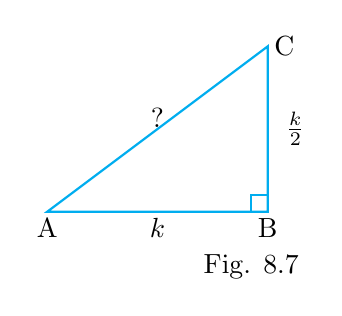
\begin{tikzpicture}[scale=0.7]
% Set up the triangle
\coordinate (A) at (0,0);
\coordinate (B) at (4,0);
\coordinate (C) at (4,3);

% Draw the triangle
\draw[thick, cyan] (A) -- (B) -- (C) -- cycle;

% Right angle mark
\draw[thick, cyan] (3.7,0) -- (3.7,0.3) -- (4,0.3);

% Labels
\node at (0,-0.3) {A};
\node at (4,-0.3) {B};
\node at (4.3,3) {C};
\node at (2,-0.3) {$k$};
\node at (4.5,1.5) {$\frac{k}{2}$};
\node at (2,1.7) {?};

% Caption
\node at (3.7,-1) {Fig. 8.7};
\end{tikzpicture}
\vspace{-10pt}
\end{wrapfigure}
\noindent If in a right triangle ABC, sin A = $\frac{1}{2}$, then that means that $\frac{\mathrm{BC}}{\mathrm{AC}} = \frac{1}{2}$, i.e., the lengths of the sides BC and AC of the triangle ABC are in the ratio 1 : 2. If the length of AC is equal to $k$, then BC will be $\frac{k}{2}$, where $k$ is any positive number. To determine other trigonometric ratios for the angle A, we need to find the length of the third side AB. Do you recall the Pythagoras theorem? Let us use it to determine the required length AB.

\begin{align*}
\mathrm{AB}^2 &= \mathrm{AC}^2 - \mathrm{BC}^2 = (k)^2 - \left(\frac{k}{2}\right)^2 = k^2 - \frac{k^2}{4} = \frac{3k^2}{4} \\
\text{Therefore,} \quad \mathrm{AB} &= \frac{\sqrt{3}k}{2} \\
\text{So, we get} \quad \mathrm{AB} &= \frac{\sqrt{3}k}{2} \quad \text{(Why is AB not $-\frac{\sqrt{3}k}{2}$?)}
\end{align*}

\noindent Now,
\begin{align*}
\cos \mathrm{A} &= \frac{\mathrm{AB}}{\mathrm{AC}} = \frac{\frac{\sqrt{3}k}{2}}{k} = \frac{\sqrt{3}}{2}
\end{align*}

\noindent Similarly, you can obtain the other trigonometric ratios of the angle A.

\vfill
\begin{center}
2019-20
\end{center}
\pagestyle{empty}
\end{document}
\documentclass[a4paper,12pt]{article}
\usepackage[utf8]{inputenc}
\usepackage{graphicx}
\usepackage{xcolor}
\usepackage{geometry}
\usepackage{enumitem}
%\usepackage{fancyhdr}
\usepackage{wrapfig}
\geometry{top=1in, bottom=1in, left=1in, right=1in}

%\cfoot{2019-20}

\definecolor{myblue}{RGB}{0,112,192}

\begin{document}

% Title section with QR code and Chapter number
\begin{center}
    \includegraphics[width=1.5cm]{qr.png} \\[1em]
    \hspace{3em}{\LARGE \textcolor{cyan}{\textbf{INTRODUCTION TO}}}\\[-0.3em]
    \vspace{1em}
   \hspace{5.9em} {\LARGE \textcolor{cyan}{\textbf{TRIGONOMETRY}}}
\hspace{15em}
\vspace{-2.7cm}
\begin{flushright}
   \begin{minipage}{0.2\textwidth}
   \hspace{4em}\framebox(50pt,50pt){\fontsize{30}{30}\selectfont\textbf{8}}
    \end{minipage}
\end{flushright}
    \noindent\textcolor{cyan}{\rule{\textwidth}{1pt}}
    \item\ \textcolor{cyan}{There is perhaps nothing which so occupies the\\
    middle position of mathematics as trigonometry.}\\
    ---\hspace{2cm} \textbf{-J.F. Herbert (1890)}
\end{center}

\vspace{1em}
{\large \textcolor{cyan}{\textbf{8.1 Introduction}}}

\vspace{0.5em}
You have already studied about triangles, and in particular, right triangles, in your earlier classes. Let us take some examples from our surroundings where right triangles can be imagined to be formed. For instance:

\vspace{1em}

% Example 1: Paragraph + Fig 8.1
\noindent
\begin{minipage}[t]{0.6\textwidth}
\raggedright
\vspace{-5cm}
\textbf{1.} Suppose the students of a school are visiting Qutub Minar. Now, if a student is looking at the top of the Minar, a right triangle can be imagined to be made, as shown in Fig. 8.1. Can the student find out the height of the Minar without actually measuring it?
\end{minipage}%
\hfill
\begin{minipage}[t]{0.35\textwidth}
\centering
\includegraphics[width=\linewidth]{fig8_1.png}\\
\textbf{Fig. 8.1}
\end{minipage}

\vspace{2em}

% Example 2: Paragraph + Fig 8.2
\noindent
\begin{minipage}[t]{0.6\textwidth}
\raggedright
\vspace{-5cm}
\textbf{2.} Suppose a girl is sitting on the balcony of her house located on the bank of a river. She is looking down at a flower pot placed on a stair of a temple situated nearly on the other bank of the river. A right triangle is imagined to be made in this situation as shown in Fig. 8.2. If you know the height at which the person is sitting, can you find the width of the river?
\end{minipage}%
\hfill
\begin{minipage}[t]{0.35\textwidth}
\centering
\includegraphics[width=\linewidth]{fig8_2.png}\\
\textbf{Fig. 8.2}
\end{minipage}

\begin{center}
2019-20
\end{center}
\pagestyle{empty}
\end{document}
	
